\providecommand{\topdir}{..}
\documentclass[../main.tex]{subfiles}

\ifSubfilesClassLoaded{
  \externaldocument[main-]{../main}
  \externaldocument[fm-]{../00_front_matter/front_matter}
  \externaldocument[intro-]{../01_introduction/introduction}
  \externaldocument[l96-]{../02_lorenz96/lorenz96}
  \externaldocument[rb-]{../03_rayleigh_benard/rayleigh_benard}
  \externaldocument[eval-]{../05_evaluation/evaluation}
  \externaldocument[conc-]{../06_conclusion/conclusion}
  \externaldocument[app-]{../07_appendix/appendix}

  \setcounterref{chapter}{main-chap:tendencies}
  \addtocounter{chapter}{-1}
}{}

\begin{document}

\ifSubfilesClassLoaded{
    \frontmatter
    \tableofcontents
    \mainmatter
}{}

\chapter{Calculation and modelling of subgrid tendencies}
\label{chap:tendencies}
\setlength{\epigraphwidth}{.45\textwidth}
\epigraphhead[0.1\textheight]{
    \epigraph{%
        Good approximations often lead to better ones.
    }{\emph{Mathematical Methods in Science}\\George P\`{o}lya, 1977}
}

\todo{introductory paragraph: why am I doing this?}


\section{Calculation of subgrid tendencies} \label{sec:calculation}
The method used to calculate the subgrid tendencies is described below and
illustrated in the form of a flowchart in \cref{fig:method}.
\begin{enumerate}
    \item\label[step]{itm:fine_model} The fine model was integrated for [\todo{}]
        time units. Every 3 time units, the model state was saved, and
        then saved again one time step later. This resulted in a dataset
        of [\todo{}] pairs of snapshots separated by 3 time units. An
        interval of 3 time units was chosen as it was the approximate
        decorrelation time of the model state (see
        \cref{app-sec:snapshot_freq}); using a shorter interval would
        mean saving redundant information.
    \item\label[step]{itm:diff} The first snapshot in each pair was subtracted
        from the second snapshot and the difference divided by the time step,
        giving the \emph{fine tendency} (i.e., the time derivative of the fine
        model state).
    \item Each snapshot in the fine tendency dataset was \emph{coarse-grained},
        reducing its spatial resolution to that of the coarse model. The
        nature of the coarse-graining algorithm warrants special attention
        and is discussed separately in \cref{sec:coarse_graining}.
    \item The same coarse-graining algorithm was applied to the first fine
        state snapshot in each pair from \cref{itm:fine_model}, producing a
        dataset of \emph{coarse states}.
    \item\label[step]{itm:coarse_model} Each coarse state was input as an
        initial condition for the coarse model, the coarse model integrated for
        one time step only, and the resulting state saved. There were now
        [\todo{}] pairs of coarse state snapshots separated by 3 time units,
        analogous to the fine state snapshots from \cref{itm:fine_model}.
    \item\label[step]{itm:coarse_tend} \cref{itm:diff} was repeated for the
        coarse state snapshots, producing a dataset of \emph{coarse tendencies}
        (i.e., the time derivatives predicted by the coarse model).
    \item\label[step]{itm:subgrid_tend} Finally, the coarse tendencies were
        subtracted from the coarse-grained fine tendencies, producing the
        \emph{subgrid tendencies}.
\end{enumerate}

\begin{figure}[ht]
    \centering
    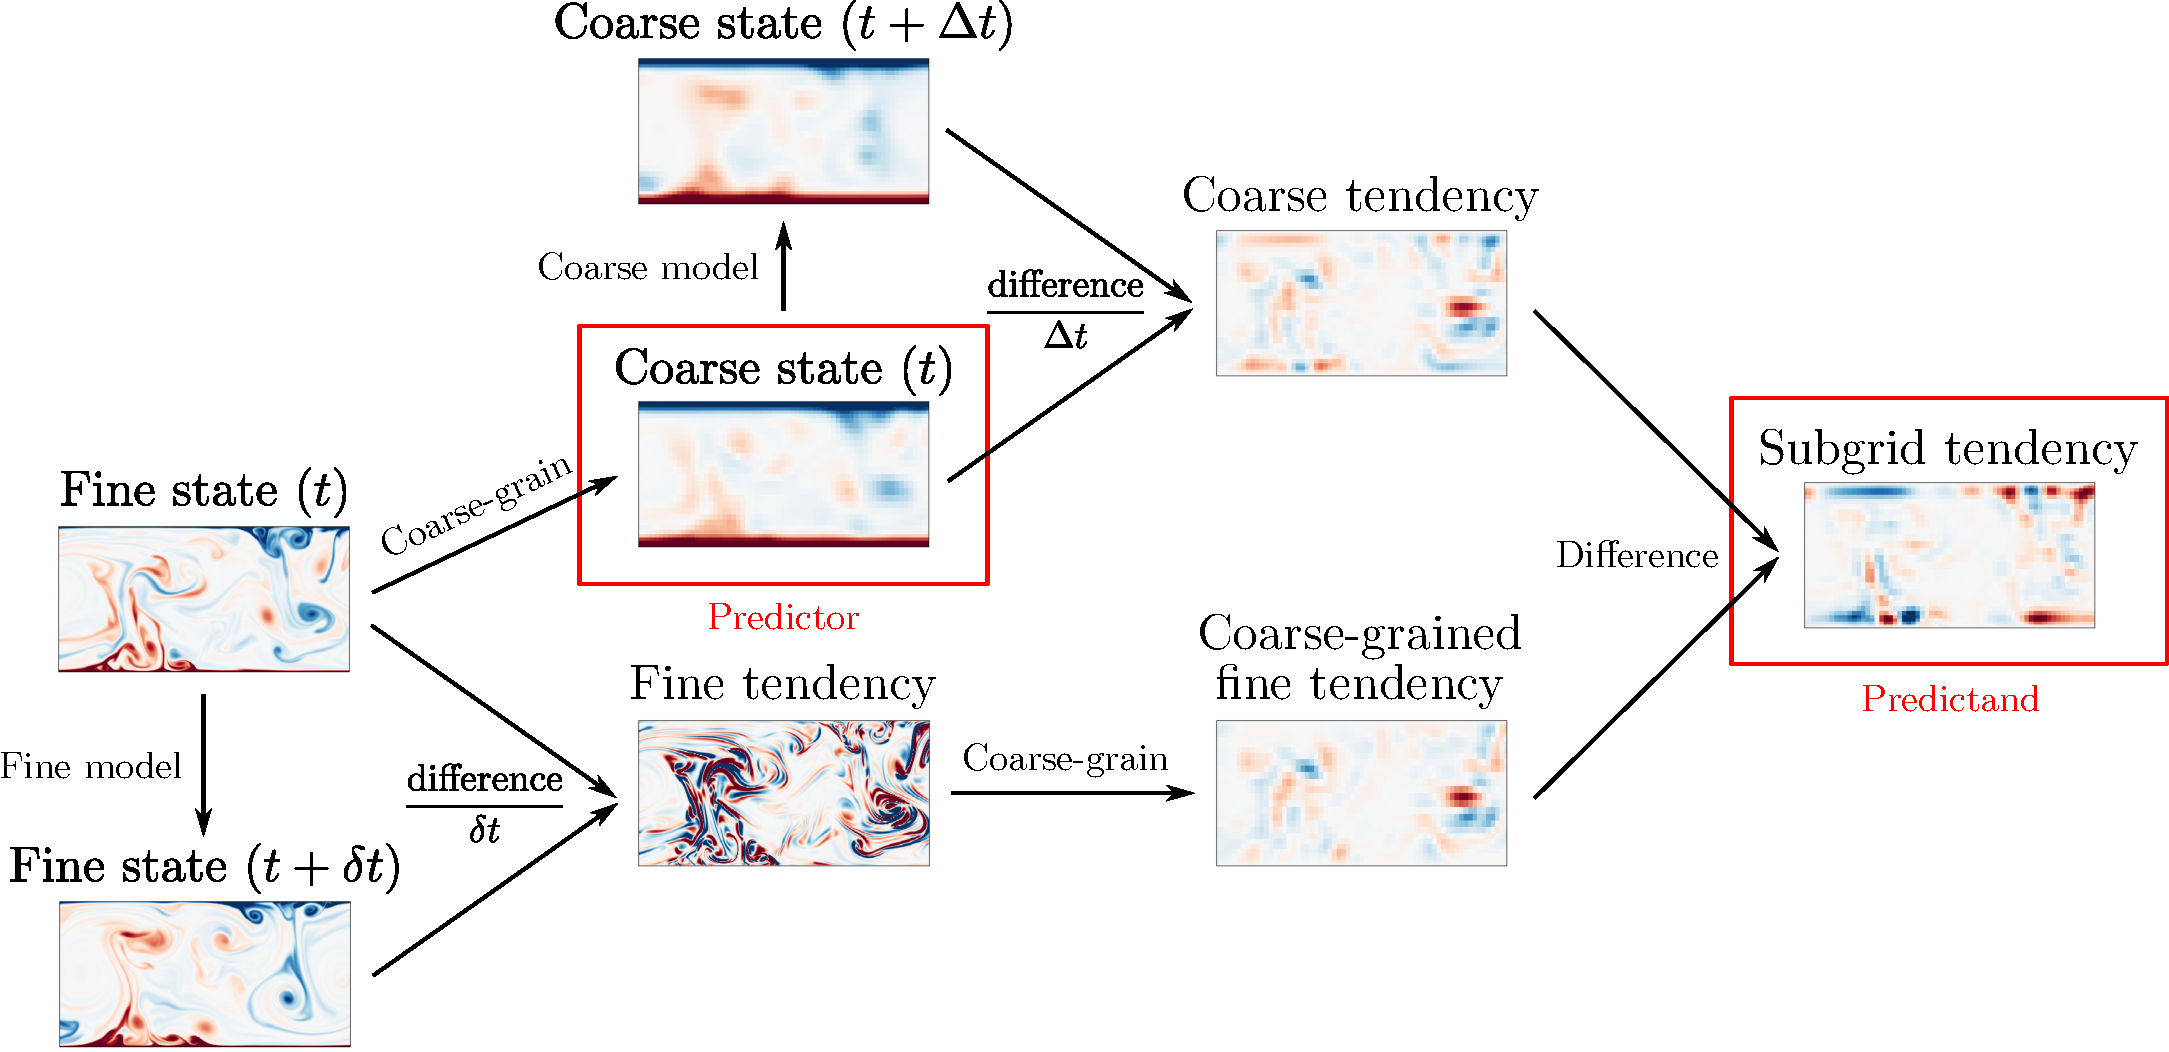
\includegraphics[width=\linewidth]{figures/method.pdf}
    \caption{
        Flowchart illustrating the procedure used to calculate
        subgrid tendencies. The plots show an example of the workflow being
        applied to the temperature data and are for illustrative purposes only.
    }
    \label{fig:method}
\end{figure}


\section{Choice of coarse-graining method} \label{sec:coarse_graining}
Coarse-graining is the process of reducing a gridded dataset onto a
lower-resolution grid, and it is required at two points in the subgrid tendency
calculation workflow: first to produce the coarse-grained fine tendency and
then to produce the coarse state. It was found that the choice of
coarse-graining method was a major influence on the quality of the calculated
subgrid tendencies; this is the consequence of a subtle issue that initially
seems purely philosophical but in fact has important practical consequences.

Broadly speaking, the output of a coarse (i.e., reduced-order) model is meant
to approximate a certain \emph{representation} of the output of the original
fine model. To give three concrete examples, the coarse model might seek to
reproduce (a) the values of the high-resolution fields on a sparser grid of
points, or (b) the averages over a set of larger grid boxes, or (c) the first
$N$ Fourier coefficients (where $N$ is less than the number of coefficients
needed to fully determine the original field). The modeller has the freedom
choose a representation, which in turn determines how the output of the coarse
model should be interpreted. The choice of representation also implicitly
determines a coarse-graining operation: a map from the state space of the fine
model to the state space of the coarse model that isolates the necessary
large-scale information and discards the rest. Referring to the previous
examples, option (a) calls for an operation that simply discards, say, three
out of every four or nine out of ten grid points. Option (b) calls for the
grouping and averaging of the grid points that lie within each large grid box.
Option (c) calls for the truncation of fine fields at the $N$th coefficient in
Fourier space.

The key lesson that was learnt during the course of this work is that the
chosen representation and coarse-graining method must be appropriate to the
nature of the coarse model. In this work, the coarse model was a Dedalus solver
that, in \cref{itm:coarse_model} of the workflow in \cref{sec:calculation},
received gridded initial condition data in real space and integrated the
governing equations forward in time using the same numerical method as the
fine model. This gave rise to two constraints on the coarse-graining method:
\begin{enumerate}
    \item The coarse-grained initial condition must be well-resolved on the
        coarse model's grid. Numerical solution algorithms for PDEs assume
        (e.g., by approximating derivatives as finite differences) that the
        solution is well-resolved on the discrete model grid, and can become
        unstable or produce output marred by artefacts if this condition is not
        met.
    \item The initial condition must respect physical constraints, namely the
        divergence-free condition \cref{rb-eqn:incompressible} and the boundary
        conditions \crefrange{rb-eqn:bc_bot}{rb-eqn:bc_sides}. A numerical
        algorithm cannot be expected to behave predictably when presented with
        unphysical initial conditions.
\end{enumerate}

During the development of this study, before the above requirements were known,
coarse-graining was performed by averaging the fine grid points that lay within
each coarse grid box (a method known within the Earth sciences as
\emph{first-order conservative regridding} because it preserves mean values).
Figure \todo{figure comparing coarse-graining methods}, illustrating the
application of first-order conservative regridding to sample temperature data,
demonstrates that the result is not very well-resolved on the coarse grid; in
many places, adjacent grid points have sharp differences in temperature.
First-order conservative regridding is also not guaranteed to preserve boundary
values or the divergence-free nature of the velocity field. Consequently, the
tendencies obtained from the coarse model in \cref{itm:coarse_tend} of the
workflow suffered from noise and numerical artefacts that propagated to
the subgrid tendencies in \cref{itm:subgrid_tend}. With the signal of interest
obscured, it was impossible to model the subgrid tendencies as functions of
the coarse state.

This issue was remedied using a new coarse-graining method. Consider the new
set of PDEs
\begin{align}
    \label{eqn:diffusion_u}
    \pdiff{\vec{u}}{t} &= -\grad \pi + \nabla^2 \vec{u}, \\
    \label{eqn:diffusion_theta}
    \pdiff{\theta}{t} &= \nabla^2 \theta, \quad \text{and} \\
    \label{eqn:diffusion_continuity}
    \grad \cdot \vec{u} &= 0,
\end{align}
subject to the required boundary conditions
\crefrange{rb-eqn:bc_bot}{rb-eqn:bc_sides}. \cref{eqn:diffusion_theta} is
simply a heat equation; over time, its initial condition is ``smoothed'', akin
to the conduction of heat through the fluid in the absence of advection.
\cref{eqn:diffusion_u} is the same except for the addition of the ``pressure''
term $-\grad \pi$, which provides an additional degree of freedom that is
needed to simultaneously enforce the divergence-free condition.
\cref{eqn:diffusion_continuity}. The properties of these equations motivated
the construction of a Dedalus model to solve them on the same grid as the
fine model.


\section{Analysis of subgrid tendencies}


\section{Modelling of subgrid tendencies}


\ifSubfilesClassLoaded{%
    \emergencystretch=5em
    \printbibliography{}
}{}

\end{document}
